\chapter{The LHC and the CMS Detector}

% **************************** Define Graphics Path **************************
\ifpdf
    \graphicspath{{Chapter3/Figs/Raster/}{Chapter3/Figs/PDF/}{Chapter3/Figs/}}
\else
    \graphicspath{{Chapter3/Figs/Vector/}{Chapter3/Figs/}}
\fi


%********************************** % First Section  *************************************
\section{The Large Hadron Collider}  %Section - 1.1 
\label{sec:detector_lhc}

The Large Hadron Collider (LHC) is a 27 km circumference proton-proton 
synchrotron accelerator with a maximum design centre of mass energy,
$\sqrt{s} = 14$ \tev. It is the highest energy component of the CERN accelerator
complex (figure~REF). The LHC accelerates counter-rotating beams of protons 
using 400 MHz radio frequency
(RF) cavities, focusses the beam using multiple quadrapole and higher order magnets,
and maintains the beams trajectory using super-conducting, niobium-titanium 
dipole magnets, capable of producing an 8.4 Tesla magnetic field. This high 
magnetic field is achieved by cooling the magnets to 1.9 K using superfluid 
helium, and applying a 11.85 kA electric current.

The beams, consisting of approximately 1400 bunches of $~1.1x10^{11}$ protons,
are brought into collision
at four points around the LHC ring within specialised detector systems. During the
first run of the LHC, `Run I', bunches were spaced in 50ns intervals, leading to
a bunch crossing rate of 20 MHz. Collisions continue for a number of hours, 
while collision rates are maintained by scanning the transverse beam positions, 
until such a time when proton numbers are depleted, the beam is dumped and the 
fill process repeated.

Simultaneous interactions happening at the time
of each bunch crossing are referred to as in-time pile up (PU), 
causing experimental challenges for detector readout and event reconstruction.

\emph{instantaneous and integrated luminosity}

The four detectors of the LHC consist of \texttt{ALICE}, \texttt{ATLAS},
\texttt{CMS} and \texttt{LHCb}. Of these, both \texttt{ATLAS} and \texttt{CMS} 
are considered as general purpose detectors, optimised for the investigation of
high-\Pt phenomena, making them ideal detectors for new physics.

The work in this thesis uses the \texttt{CMS} detector, which is discussed in 
the following section.


%********************************** % Second Section  *************************************
\section{Compact Muon Solenoid}  %Section - 1.2 
\label{sec:detector_overview}

CMS, standing for `Compact Muon Solenoid' (figure~\ref{fig:cms_diagram}), is a
hermetic detector system 
optimised for the study on high-\Pt objects and their decays, produced in the 
proton collisions at the LHC. It is designed to make accurate measurements of 
the positions and momenta of physics objects such as electrons, muons, taus, 
photons and jets. Owing to an almost complete 4$\pi$ solid angle coverage, CMS is 
capable of also making accurate measurements of global energy imbalances due to 
the presence of weakly interacting particles.

\begin{figure}[hb!]
  \centering
  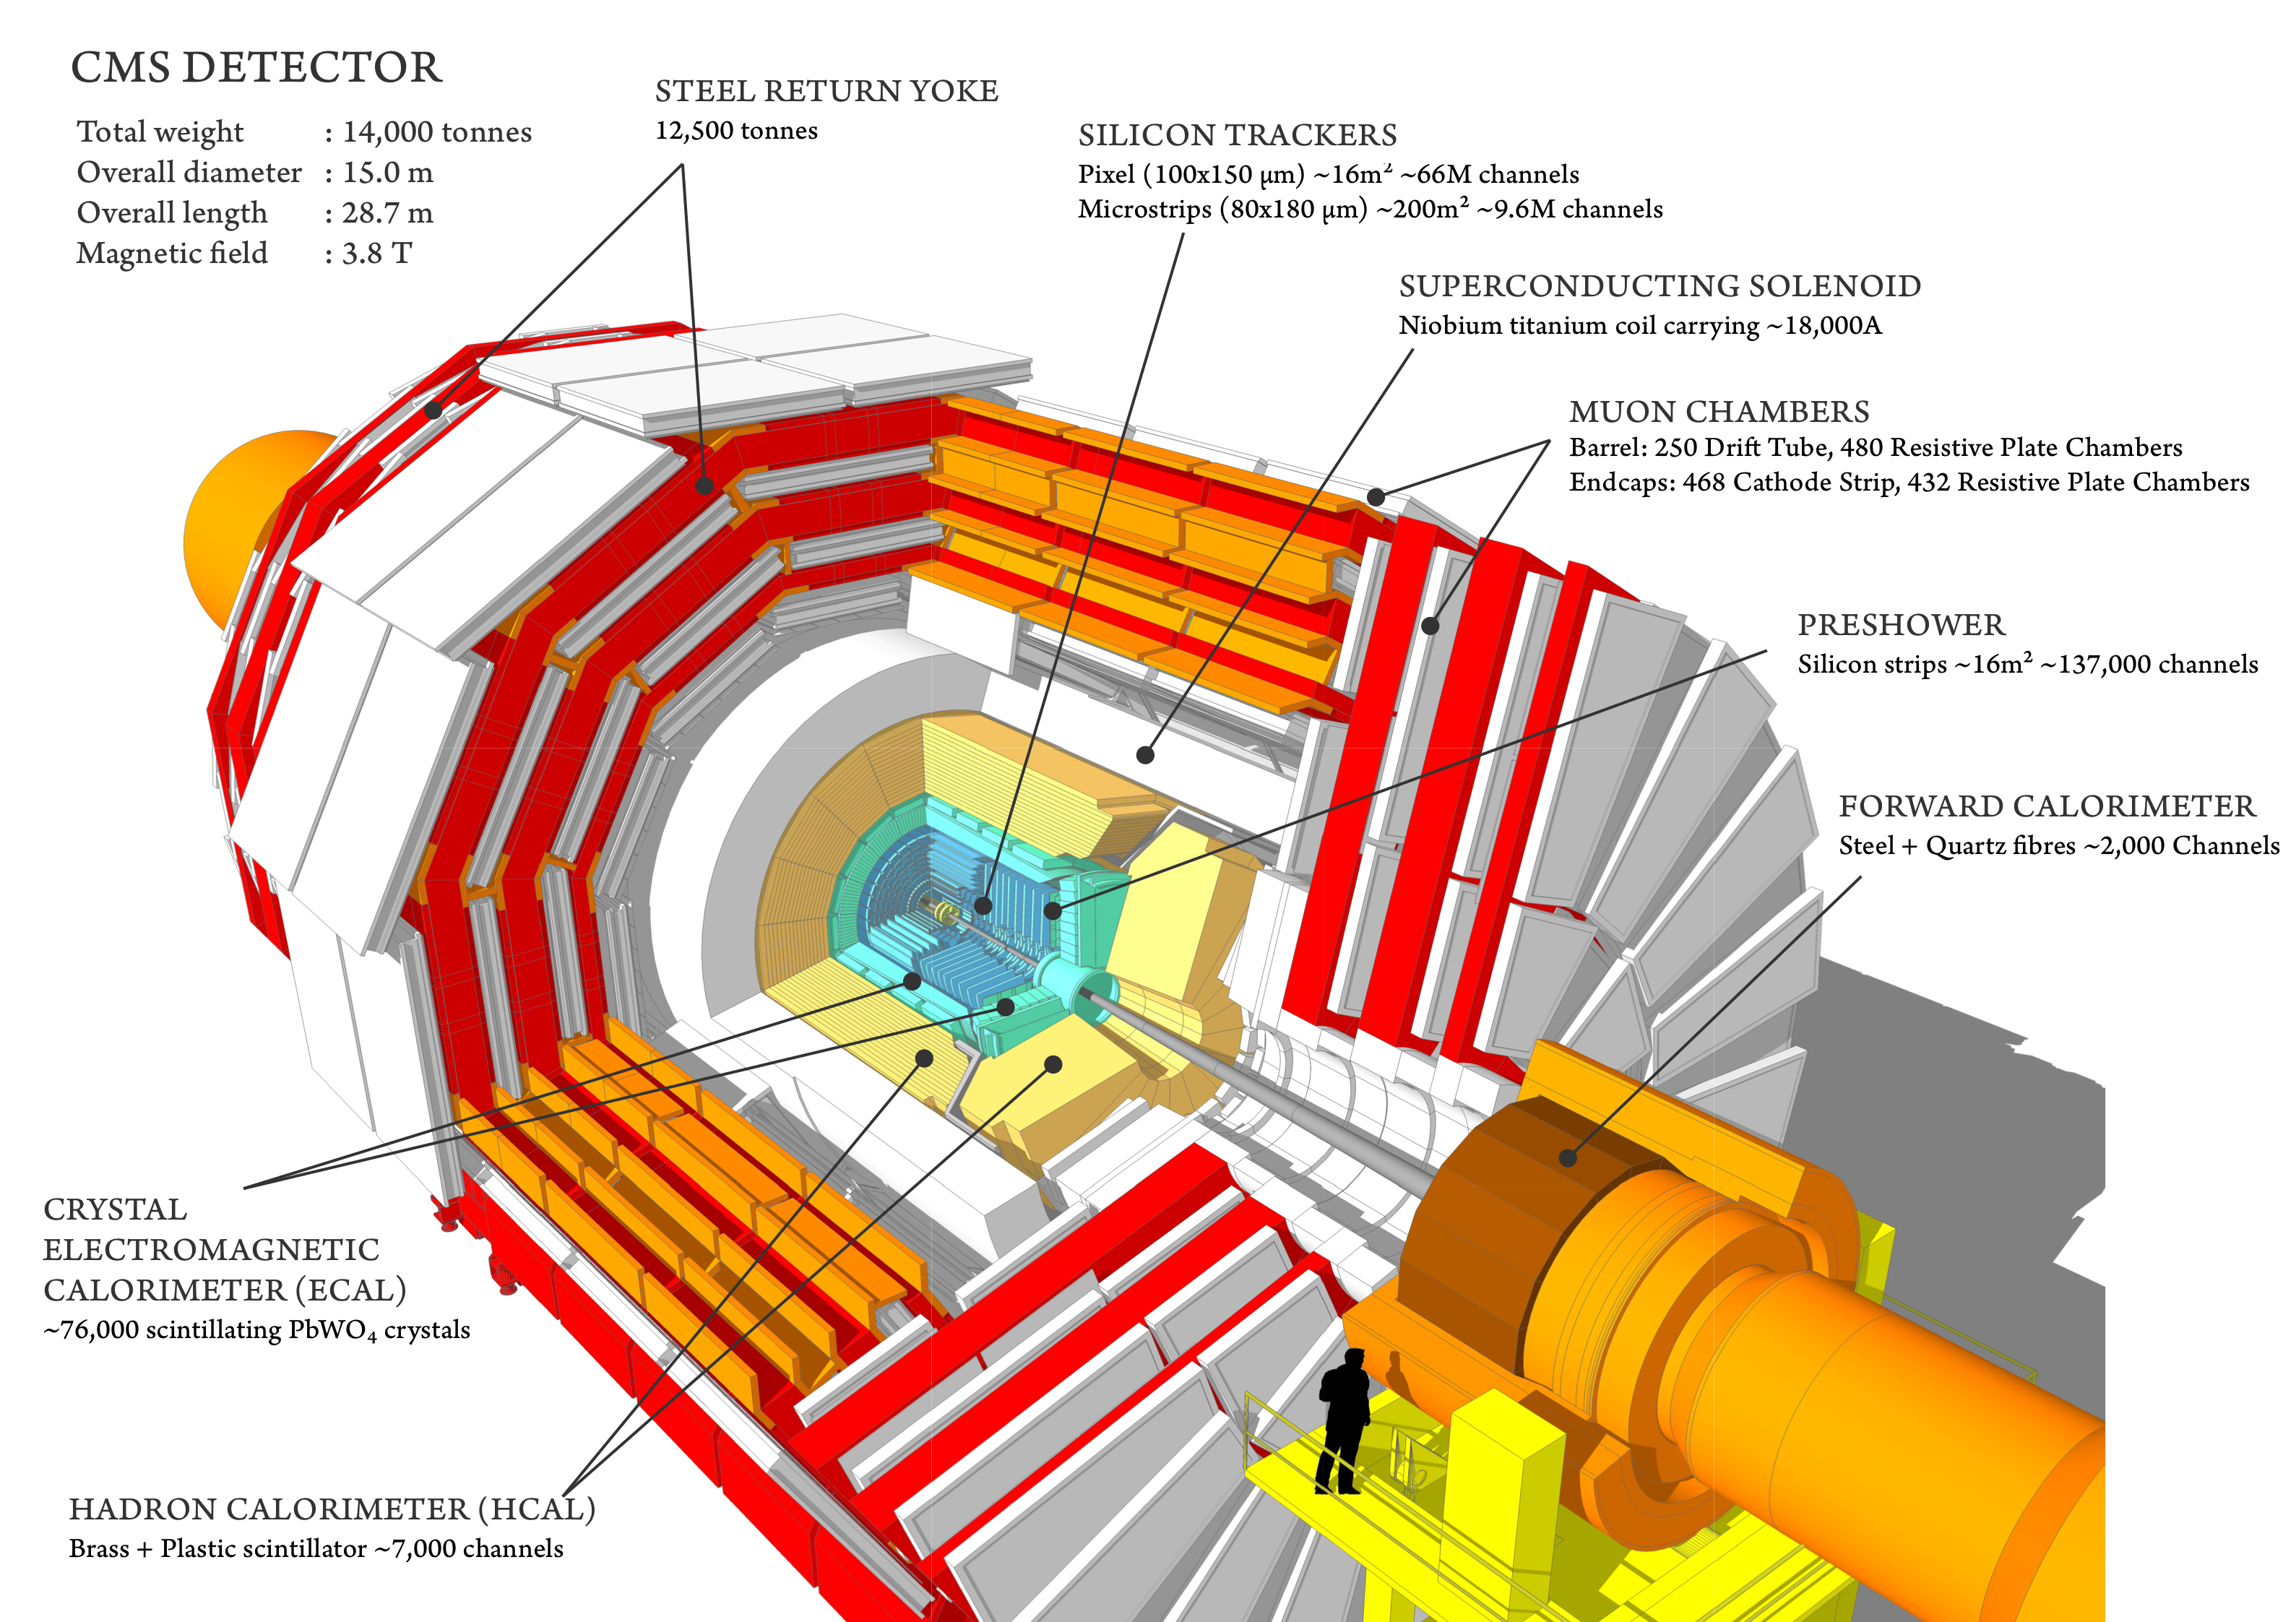
\includegraphics[width=\textwidth]{Figs/cms_120918_02.png}
  \caption{Diagram of the Compact Muon Solenoid REF.}
  \label{fig:cms_diagram}
\end{figure}

The cylindrical detector is 28 m in length, 15 m in diameter and has a mass of 
around 14,000 tonnes \footnote{if it was placed in the bath, it would sink.}. 
The z-axis is taken to be the longitudinal dimension along the beamline, the x-
axis the perpendicular direction pointing towards the centre of the LHC ring, 
and the y-axis pointing skywards, perpendicular to these forming a right-handed 
co-ordinate system. The transverse plane is taken to be the plane of the x and y
axes.

Directions relative to the CMS detector are described with the variables $\phi$,
the angular direction in the transverse plane with the range $[-\pi, \pi]$, and 
the pseudo-rapidity, $\eta$, describing the angle with respect to the z-axis,
defined as:

\begin{equation}
\eta = - ln \Bigg[ tan \Bigg( \frac{\theta}{2} \Bigg) \Bigg]
\end{equation}

where blah blah. Differences in these two variables, $\Delta \phi$ and $\Delta 
\eta$, are invariant under Lorentz boosts, and so can be used to construct a 
furthermore Lorentz-invariant angular seperation between particles:

\begin{equation}
\Delta R = \sqrt{ (\Delta \eta)^2 + (\Delta \phi)^2}
\end{equation}

CMS is arranged in a layered configuration of sub-detectors, structured as a 
cylindical barrel, `closed' by two endcaps.

\emph{discuss the magnet here.}

%********************************** % Third Section  *************************************
\section{Detector Subsystems}  %Section - 1.3
\label{sec:detector_subsystems}

Detector subsystems within CMS follow a layered structure in both the barrel and
endcap regions. The following describe each of the subsystems in more detail.

\subsection{Pixels and tracker}
- inner three layers of pixel detectors
    - also have endcaps of pixel detectors
- what type of pixels? what pitch? technology?
- provide 2d information of hit positions

- further 10 layers of silicon strip detectors
    - n-in-p?
    - and endcaps

- this detector system provides information of not only the vertex location and 
tracking of charged particles, but also given the massive magnet, a 
determination of both their charge and momenta.

\subsection{Electromagenetic Calorimeter}

- ecal made of scintillating lead tungstate (PbWO4) crystals
    - each crystal is 0.017 x 0.017 (in deltaEta x deltaPhi dimensions), and 23 
    cm in length
        -   corresponds to about 25 radition lengths
        - moliere radius?
    - super-crystal arrangement?
- each crystal has a photodetector to determine the level of scintillation light
produced
    - avalanche photo-diodes in the barrel, and vacuum photo-triodes in the 
    endcap region
    - radiation hardness?
    - what material?

- this detector system provides energy and spatial information of
electromagnetically showering particles.

\emph{can i ignore the pre-shower rubbish, as we don't consider endcap objects? 
- or do we for electromagnetic particles?!}

\subsection{Hadronic Calorimeter}

- alternating layers of brass absorber and plastic scintillator
- scintillators are sectioned into towers, 0.087x0.087 in barrel and 0.17x0.17 
in the endcaps (double check this isn't just my interpretation of ted's eta 
numbers)
- light produced in the scintillator layers is transmitted via wavelength 
shifting fibres to a hybrid photo-diode for detection

\emph{can i ignore the HF region, as we ignore forward jets?}

\subsection{Muon Systems}

%********************************** % Fourth Section  *************************************
\section{Trigger and Data Acquisition}  %Section - 1.4
\label{sec:detector_daq}

\subsection{Trigger system}

\subsubsection{Level-1 Hardware Trigger}

\subsubsection{High-level Trigger}

\subsection{DAQ system}

